\documentclass[a4paper,12pt]{article}
\usepackage{tikz}
\usepackage{caption}
\usepackage{listings}
\lstset{keywordstyle=\sffamily\color{red},basicstyle=\fontsize{11}{12}\selectfont\ttfamily}

\usetikzlibrary{positioning}
\usetikzlibrary{shapes.geometric, arrows}
\tikzstyle{startstop} = [rectangle, rounded corners, minimum width=3cm, minimum height=1cm,text centered, draw=black, fill=red!30]
\tikzstyle{io} = [trapezium, trapezium left angle=70, trapezium right angle=110, minimum width=3cm, text width=3cm, minimum height=1cm, text centered, draw=black, fill=blue!30]
\tikzstyle{process} = [rectangle, minimum width=3cm, minimum height=1cm, text centered, text width=3cm, draw=black, fill=orange!30]
\tikzstyle{decision} = [diamond, minimum width=3cm, minimum height=1cm, text centered, text width=1.5cm, draw=black, fill=green!30]
\tikzstyle{arrow} = [thick,->,>=stealth]

\begin{document}
\section*{Second use case: Bringing objects from another person}
The use case which should be implemented can be described as follows: Hobbit should be repetitively asking User A if it should bring an object from User B, which is located at another place. First the user should be asked which objects should be picked up (e.g. "Which object do you want?"). User A then should use the robot’s tablet to enter the name of the requested object. After that, Hobbit should navigate to the User B. User B then should be asked to handover the desired object. If it is answerd positively, the object should be placed on Hobbit's tray and the robot navigates back to its previous location telling User A "Here you are" and placing the object on the table. If the object has not been handed over, an appropriate message should be displayed on the tablet (e.g. "I’m sorry, your partner couldn’t handover the object") after navigating back.

Afterwards User A should be asked, if Hobbit should bring another item. The whole procedure should be performed as long as User A does not request any other object. After the final decline Hobbit should show a happy emotion. For a better understanding figure \ref{fig:SecondUserCaseFlow} provides the flowchart of this use case. The locations of User A and B can be consired as the following poses:

\begin{itemize}
    \item User A:
    \begin{itemize}
        \item \lstinline!position:{x:1.0,y:2.0,x:0.0}!
        \item \lstinline!orientation:{x:0.0,y:0.0,z:0.0,w:1.0}!
    \end{itemize}
    \item User B:
    \begin{itemize}
        \item \lstinline!position:{x:14.0,y:-5.0,x:0.0}!
        \item \lstinline!orientation:{x:0.0,y:0.0,z:0.0,w:0.6}!
    \end{itemize}
\end{itemize}

Please implement a solution using the Blockly editor, which lets Hobbit show the desired behaviour, with respect to the following conditions:
\begin{itemize}
    \item Start working by clicking the "Start" button of the interface
    \item Do not close the graphical editor during your work
    \item Click the "Stop" button when you finished implementation
    \item Click "Submit" to submit your solution
    \item Each block provides a help page - it is accessible via \textit{right click} $\rightarrow$ \textit{Help}
\end{itemize}

\begin{figure}[!htbp]
	\centering
    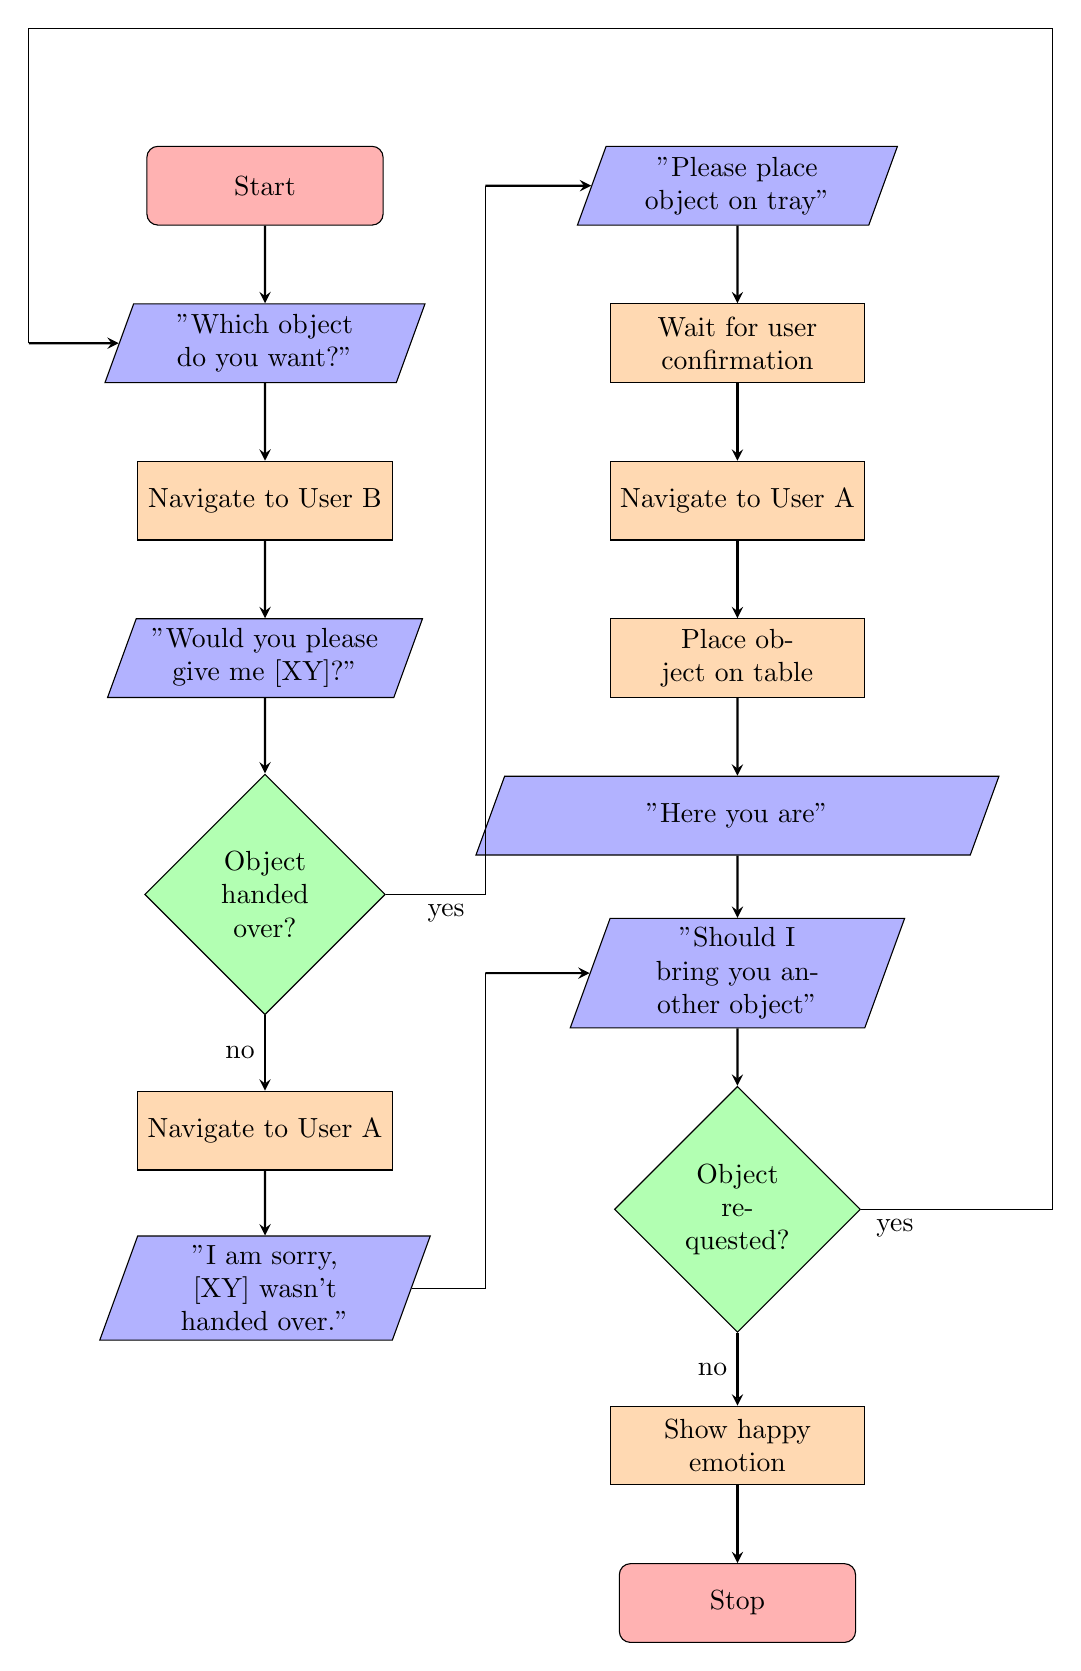
\begin{tikzpicture}[node distance=2cm]
        \node (start) [startstop] {Start};
        \node (in1) [io, below of=start,] {"Which object do you want?"};
        \node (pro1) [process, below of=in1] {Navigate to User B};
        \node (out1) [io, below of=pro1] {"Would you please give me [XY]?"};
        \node (dec1) [decision, below of=out1, yshift=-1cm] {Object handed over?};
        \node (pro3) [process, below of=dec1, yshift=-1cm] {Navigate to User A};
        \node (out2) [io, below of=pro3] {"I am sorry, [XY] wasn't handed over."};
        \node (out3) [io, right of=start, xshift=4cm] {"Please place object on tray"};
        \node (pro4) [process, below of=out3] {Wait for user confirmation};
        \node (pro5) [process, below of=pro4] {Navigate to User A};
        \node (pro6) [process, below of=pro5] {Place object on table};
        \node (out4) [io, below of=pro6] {"Here you are"};
        \node (out5) [io, below of=out4] {"Should I bring you another object"};
        \node (dec2) [decision, below of=out5, yshift=-1cm] {Object requested?};
        \node (pro7) [process, below of=dec2, yshift=-1cm] {Show happy emotion};
        \node (stop) [startstop, below of=pro7] {Stop};
        \draw [arrow] (start) -- (in1);
        \draw [arrow] (in1) -- (pro1);
        \draw [arrow] (pro1) -- (out1);
        \draw [arrow] (out1) -- (dec1);
        \draw [arrow] (dec1) -- node[anchor=east] {no} (pro3);
        \draw [arrow] (pro3) -- (out2);
        \draw (out2) -| (2.8,-10);
        \draw [arrow] (2.8,-10) -- (out5);
        \draw (dec1) -| node[anchor=north, xshift=-0.5cm] {yes} (2.8,0);
        \draw [arrow] (2.8,0) -- (out3);
        \draw [arrow] (out3) -- (pro4);
        \draw [arrow] (pro4) -- (pro5);
        \draw [arrow] (pro5) -- (pro6);
        \draw [arrow] (pro6) -- (out4);
        \draw [arrow] (out4) -- (out5);
        \draw [arrow] (out5) -- (dec2);
        \draw [arrow] (dec2) -- node[anchor=east] {no} (pro7);
        \draw [arrow] (pro7) -- (stop);
        \draw (dec2) -| node[anchor=north, xshift=-2cm] {yes} (10,2);
        \draw (10,2) -| (-3,-2);
        \draw [arrow] (-3,-2) --  (in1);
    \end{tikzpicture}
    \caption{Flowchart of second use case} \label{fig:SecondUserCaseFlow}
\end{figure}

\end{document}